\documentclass[10pt]{article}
\usepackage{icmlko}

\icmlmeta{IP 파운데이션 월드모델}{126}{안쪽은 평평했다}{한 도메인의 이력만으로 정해지는 모수는 기간 안에서 검증되고 지평 너머에서 배신한다 --- 서로 다른 기제 셋이 같은 부호로 뒤집혔다}

\begin{document}

\twocolumn[
\icmlheader

\begin{abstract}
노트 125가 만든 하네스에 도전자 일곱을 붙였다 --- 결합 위계 잠재 모형,
anchor regression, 부스팅, 짝 순위 우도, 도메인별 수축, 축 합집합 둘.
그러는 동안 서로 다른 자리에서 \textbf{같은 모양이 세 번} 나왔고, 그게
이번 노트의 본론이다. \textbf{한 도메인의 이력만으로 정해지는 모수는 학습
기간 안에서는 도움이 되고 지평 너머에서는 해가 된다.} 게임에 게임 전용 축
넷을 더하면 기간 안 $+$0.027, 지평 너머 $-$0.038. 웹툰에 자기 이력을 절반
섞으면 기간 안 $+$0.016, 지평 너머 $-$0.210. 웹툰에 도메인별 적재를 주면
기간 안 $+$0.004, 지평 너머 $-$0.359. 기제가 셋 다 다른데 부호가 셋 다
같다. 풀링된 모수는 아홉 도메인이 같이 정하니 한 도메인이 흔들려도 덜
움직이고, 도메인 고유 모수는 그 도메인의 표류에 그대로 노출된다.
\textbf{따름정리가 아프다} --- 학습 기간 안에 갇힌 어떤 검증 절차도 이걸
못 잡는다. 교차검증은 도메인 고유 구조를 \emph{지지}한다. 기간 안에서는
실제로 맞으니까. 웹툰의 배합비는 안쪽에서 폭 0.034로 평평한데 바깥에서는
$+$0.236에서 $-$0.191까지 0.43을 간다. 검증 창을 겹치게 잡았던 탓에 그
0.034가 $t$ 검정까지 통과했고, 창을 갈라 놓아도 재현됐다 --- 잡음이 아니라
2025년에 관계가 달라진 것이다. 그래서 문턱을 고르는 자료가 아니라
\emph{표류량}에서 끌어왔다. 학습 기간 안에서 관계가 해마다 얼마나
움직이는지(중앙 0.110/년) 재고 지평 1.5년을 곱한 0.1655를 못 넘는 이득에는
도메인 고유 구조를 사지 않는다. 곁가지로 둘을 더 고쳤다. \textbf{상각 격차}
--- 잠재 변수를 학습에서는 자유 모수로 두고 예측에서는 능형으로 풀고
있었다. 양쪽을 같은 풀이로 맞추자 $+$0.1009에서 $+$0.3517로 올랐다.
\textbf{$z$는 가드지 순위가 아니다} --- 부스팅이 판 $\rho$로는 F6 · F9 ·
F10보다 낮은데 $z$는 전부보다 높게($+$4.41) 나왔다. 규제가 세면 섞인
라벨도 못 맞혀 귀무가 좁아진다.
\end{abstract}
]

\begin{figure*}[t]
\centering
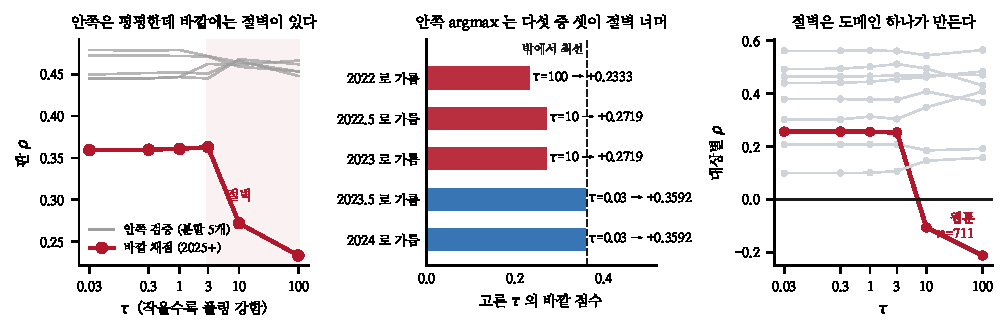
\includegraphics[width=\textwidth]{figs/tau.pdf}
\caption{왼쪽 --- 안쪽 검증 곡선 다섯은 평평한데 바깥에는 $\tau$ 3과 10
사이에 절벽이 있다. 가운데 --- 그래서 안쪽 argmax는 다섯 중 셋이 절벽
너머를 집는다. 오른쪽 --- 그 절벽은 도메인 하나(웹툰, $n$=711)가 만든다.}
\end{figure*}

\section{같은 법칙이 세 번 나왔다}

도전자 일곱을 붙이는 동안 서로 다른 자리에서 같은 모양이 세 번 나왔다.
셋 다 ``한 도메인의 이력만으로 정해지는 모수''를 늘린 것이고, 셋 다
학습 기간 안에서는 도움이 되고 그 너머에서는 해가 됐다.

\begin{table}[t]
\centering\tsize
\caption{기제는 다르고 부호는 같다. 셋 다 학습 기간 안에서 검증을 통과하고
지평 너머에서 뒤집힌다.}
\begin{tabular}{lrr}
\toprule
& 기간 안 & 지평 너머 \\
\midrule
게임 전용 축 넷을 더함 & $+$.0273 & $-$.0384 \\
웹툰에 자기 이력 절반 & $+$.0161 & $-$.2101 \\
웹툰에 도메인별 적재 & $+$.0037 & $-$.3591 \\
\bottomrule
\end{tabular}
\end{table}

\claimx{\textbf{한 도메인의 이력만으로 정해지는 모수는 그 도메인의 표류에
그대로 노출된다.} 풀링된 모수는 아홉 도메인이 같이 정하니 한 도메인이
흔들려도 덜 움직인다. 그래서 도메인 고유 구조는 \emph{기간 안에서 진짜로}
도움이 되고 --- 그 안에서는 표류가 아직 안 일어났으니까 --- 지평 너머에서만
값을 치른다.}{셋 다 같은 자료의 같은 시간 분할 한 판이다. 부호가 셋 다
같다는 것이 우연일 확률은 낮지만, 다른 분할에서 다시 재야 한다.}

\textbf{따름정리.} 학습 기간 안에 갇힌 어떤 검증 절차도 이것을 못 잡는다.
교차검증은 도메인 고유 구조를 \emph{지지}할 것이다 --- 기간 안에서는
실제로 맞으니까. 노트 125의 F1이 왜 정렬 기구를 다 갖추고도 아무것도
못 샀는지가 여기서 설명된다. 그것도 같은 종류의 모수였다.

\section{일곱을 붙였다}

노트 125의 하네스는 정식화에 딱 하나를 요구한다 --- (도메인, 축, 마스크,
시간)에서 점수 벡터로. 그래서 성격이 다른 일곱을 한꺼번에 올렸다.
$^{*}$는 하이퍼모수를 고르느라 바깥 점수를 본 것이다(뒤의 회계 참고).

\begin{table}[t]
\centering\tsize
\caption{도전자 일곱. 전부 같은 하네스로 채점된다.
판 $\rho$는 배포 규약, $T$=2025.0.}
\begin{tabular}{llr}
\toprule
& & 판 $\rho$ \\
\midrule
F9 & 짝 순위 우도 (Bradley--Terry) & $+$.3464 \\
F10 & 도메인별 수축 & $+$.3452\rlap{$^{*}$} \\
F6 & 직접 풀링 (노트 125의 챔피언) & $+$.3413 \\
F8 & 부스팅 --- F6과 같은 자질 & $+$.3363 \\
F12 & 짝 순위 우도 $+$ 축 합집합 & $+$.3308 \\
F11 & 직접 풀링 $+$ 축 합집합 & $+$.3271 \\
F7 & anchor regression & $+$.2820 \\
\midrule
F2 & 결합 위계 잠재 & $+$.3592\rlap{$^{*}$} \\
\bottomrule
\end{tabular}
\end{table}

F8은 목적이 성능이 아니라 진단이었다. F6과 \emph{완전히 같은 자질}에
비선형 모형을 얹어서, 병목이 모형인지 축인지 가른다.

\claimx{\textbf{병목은 축이다.} F8 부스팅이 F6 선형보다 낮다 ($+$0.3363 대
$+$0.3413). 같은 자질에서 비선형이 아무것도 못 더한다면 남은 여지는 모형
쪽이 아니라 자질 쪽에 있다.}{한 종류의 비선형(히스토그램 부스팅) 한 벌의
하이퍼모수다. 다른 계열이 다를 수 있다.}

F9는 목적함수를 판정치에 맞춘 것이다. 판정치는 스피어만인데 지금껏 제곱오차로
맞춰 왔다. 도메인 안에서 짝을 뽑아 차이에 로지스틱을 태우면
(Bradley--Terry) 도메인 간 눈금 차이가 자동으로 빠진다 --- \emph{도메인
표시자조차 필요 없다.} 판 $\rho$ $+$0.3464로 F6을 넘었다.

\subsection{축을 늘려도 안 오른다 --- 그리고 왜 안 오르는지}

F8이 ``병목은 축''이라 했으니 축을 늘려 봤다. 게임에는 실은 공통 다섯 말고
전용 축이 넷 더 있다(가격 · 연령등급 · 램 · 카테고리 수). 옛 코드가 공통
다섯을 하드코딩해 그 넷을 조용히 버리고 있었다.

\claimx{\textbf{버리는 쪽이 나았다.} 축 합집합을 쓰면 판 $\rho$가
$+$0.3413에서 $+$0.3271로 내리고, \emph{특히 게임 자신이} $+$0.5473에서
$+$0.3798로 내린다. 게임 전용 축의 계수는 게임의 이력 하나로만 정해지기
때문이다 --- 기간 안 교차에서는 $+$0.2820에서 $+$0.3425로 오르고, 지평
너머에서는 $+$0.3340에서 $+$0.2956으로 내린다.}{게임에만 있는 축 넷의
사례 하나다. 다른 도메인에 전용 축을 붙여 보면 다를 수 있다.}

그러니 ``축을 늘린다''는 처방은 조건이 붙는다. \textbf{한 도메인에만 있는
축은 도움이 안 된다.} 노트 124가 연 길 --- 팝업의 빈 260건을 매기는 것 ---
이 값진 이유가 여기서 분명해진다. 그건 새 축을 만드는 게 아니라 \emph{이미
전 도메인이 공유하는 축}의 빈칸을 메우는 일이다.

\section{상각 격차 --- 학습과 예측이 다른 규칙이면 모형이 아니다}

F2는 노트 5부터 적어만 두고 한 번도 안 맞춘 식이다.
\[
\min \sum_d \bigl\| M_d \odot (X_d - \eta_d \Lambda_d^{\!\top}) \bigr\|_F^2
 + \frac{1}{\tau}\sum_d \bigl\| \Lambda_d - \bar\Lambda \bigr\|_F^2
 + w \sum_d \ell(y_d, \eta_d \beta + b_d)
\]
F1은 도메인마다 따로 분해한 뒤 \emph{사후에} 회전을 맞춘다. 그래서 정렬은
라벨을 못 보고 라벨은 정렬을 못 고친다. 여기서는 적재가 재구성과 예측
양쪽에서 같이 정해지고 $\tau$가 도메인 간 거리를 조인다.

처음 판은 형편없었다 --- 판 $\rho$ $+$0.1009. 원인이 식이 아니라 구현에
있었다.

\claimx{\textbf{학습에서는 $\eta$를 자유 모수로 두고 예측에서는 능형으로
풀고 있었다.} 그러면 학습이 최적화한 $\eta$와 예측이 만드는 $\eta$가 다른
물건이다. 양쪽 다 관측된 축에서 능형으로 풀도록 고치니 $+$0.1009에서
$+$0.3517로 올랐다.}{선형 풀이를 통과하는 역전파라 MPS에 후방 연산이 없어
CPU로 돌린다. 다만 $P$=5, $k\le5$라 GPU로 갈 이유도 없다.}

\begin{figure*}[t]
\centering
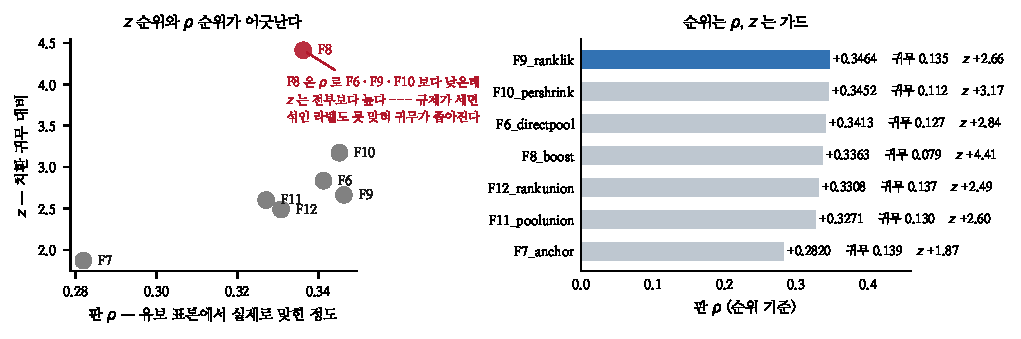
\includegraphics[width=\textwidth]{figs/rank.pdf}
\caption{왼쪽 --- $z$ 순위와 $\rho$ 순위가 어긋난다. F8은 $\rho$로 F6 · F9 ·
F10 아래인데 $z$는 전부 위다. 오른쪽 --- 순위를 $\rho$로 되돌린 표.}
\end{figure*}

\section{$z$는 가드지 순위가 아니다}

노트 125에서 순위 기준을 팝업 원점수에서 치환 귀무 대비 $z$로 옮겼다.
이번 판이 그 선택을 반증했다.

\claimx{\textbf{$z$로 줄을 세우면 규제가 셀수록 이긴다.} F8 부스팅의 귀무
폭은 0.0789로 F6의 0.1266보다 훨씬 좁다. 트리 모형은 섞인 라벨에서 평균으로
수축해 버리니 우연히 잘 보일 길이 적다. 그래서 판 $\rho$로는 F6 · F9 ·
F10 아래인데 $z$는 $+$4.41로 전부 위다. $z$는 ``우연보다 나은가''를 재는 검정통계량이지
``얼마나 잘 맞히는가''가 아니다.}{노트 125의 F1 대 F6 비교 자체는 유효하다
--- 둘은 $\rho$가 같았고($+$0.3400 대 $+$0.3413) 그때 귀무 폭이 동점을
갈랐다. 틀린 것은 그 도구를 \emph{일반 순위}로 승격시킨 것이다.}

고쳐 놓은 규칙은 이렇다. 순위는 유보 표본의 판 $\rho$. $z$는 통과/탈락
($p\le.05$). $\rho$ 차이가 대상별 짝지은 1 SE 안이면 귀무가 좁은 쪽.

\section{안쪽은 평평했다}

법칙을 처음 만난 자리는 하이퍼모수를 고르는 곳이었다.


F2의 $\tau$를 밖에서 고르면 그건 채점 자료를 본 것이다. 그래서 학습 기간을
다시 갈라 안쪽에서 골랐다. 그러자 이 판의 진짜 한계가 보였다.

\begin{table}[t]
\centering\tsize
\caption{웹툰 --- 배합비 $w$에 따른 안쪽 곡선과 바깥 곡선.
$w$=0이 완전 풀링, 1이 자기 이력만.}
\begin{tabular}{lrrrrr}
\toprule
$w$ & 0.00 & 0.25 & 0.50 & 0.75 & 1.00 \\
\midrule
안쪽 & $+$.481 & $+$.500 & \textbf{$+$.511} & $+$.498 & $+$.477 \\
바깥 & \textbf{$+$.236} & $+$.145 & $+$.025 & $-$.100 & $-$.191 \\
\bottomrule
\end{tabular}
\end{table}

\claimx{\textbf{안쪽이 평평하다는 것은 ``아무래도 좋다''가 아니라 ``여기서는
아무것도 모른다''는 뜻이다.} 웹툰의 안쪽 곡선은 폭 0.034로 평평한데 바깥
곡선은 $+$0.236에서 $-$0.191까지 0.43을 간다. 부호가 바뀐다.}{모바일은
정반대다 --- 안쪽 폭 0.591로 가파르고 바깥도 같은 방향이다. 안쪽이 가파를
때는 믿어도 된다.}

$\tau$ 쪽도 같은 모양이다. 안쪽 다섯 분할의 점수는 전부
0.445$\sim$0.479 사이인데 바깥에는 $\tau$ 3과 10 사이에 절벽이 있다
($+$0.3628 $\to$ $+$0.2719). 안쪽 argmax는 다섯 중 셋이 절벽 너머를 집는다.
그 절벽은 웹툰 하나가 만든다 --- $\tau$가 커져 도메인이 자기 적재를 갖는
순간 웹툰만 $+$0.253에서 $-$0.106으로 뒤집히고 나머지 여덟은 오히려 오른다.

\section{겹친 창은 검정이 아니다}

평평함을 잡으려고 짝지은 $t$ 검정을 걸었다. 웹툰이 통과했다.

\claimx{\textbf{검증 창을 겹치게 잡은 것이 잘못이었다.} 처음엔 각 분할이
``자른 시점 이후 전부''를 검증했다. 그러면 2022.5 분할의 검증 집합이
2023.0 분할의 검증 집합을 통째로 품는다. 분할들이 거의 같은 자료를 보니
짝지은 표준오차가 터무니없이 작아지고, 웹툰의 이득 0.016조차 유의해진다.
창을 반년씩 갈라 겹치지 않게 하자 게임이 바로잡혔다 ($+$0.334 $\to$
$+$0.544).}{훈련 집합은 여전히 중첩된다(전부 ``자른 시점 이전''). 검증
집합만 갈랐다.}

그런데 창을 갈라도 웹툰은 여전히 $w$=0.5를 고른다. 안쪽 이득 0.030이
\emph{재현}된다.

\claimx{\textbf{그러므로 이것은 잡음이 아니다.} 웹툰의 축$\to$라벨 관계가
2025년에 달라졌고, 2025년 이전 자료는 그것을 볼 방법이 없다. 검증 창 뒤에
오는 체제 변화는 어떤 교차검증으로도 안 잡힌다.}{``2025년에 달라졌다''는
관측이지 설명이 아니다. 웹툰 쪽에 무슨 일이 있었는지는 이 자료로 모른다.}

\begin{figure*}[t]
\centering
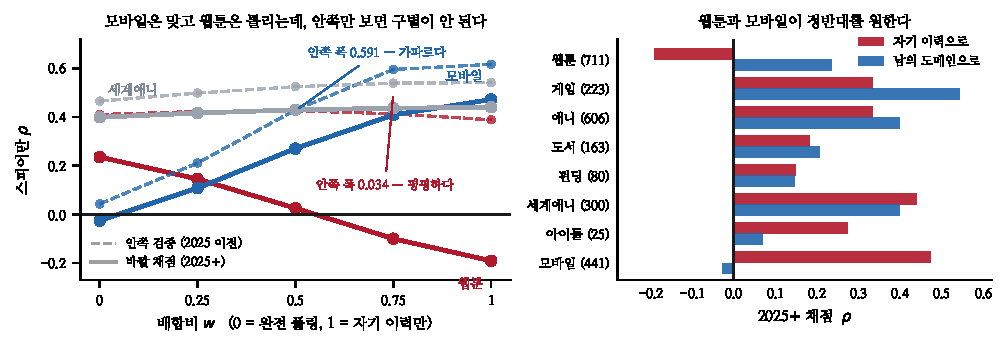
\includegraphics[width=\textwidth]{figs/decay.pdf}
\caption{왼쪽 --- 배합비를 안쪽에서 본 곡선과 바깥에서 본 곡선. 모바일은
맞고 웹툰은 틀리는데, 안쪽만 보면 그 차이를 알 길이 없다.
오른쪽 --- 자기 이력으로 맞힌 것과 남의 도메인으로 맞힌 것.}
\end{figure*}

\section{문턱을 표류에서 끌어오다}

절대 문턱을 손으로 정하면 그것도 결국 바깥을 본 것이다. 대신 독립된
측정에서 끌어왔다.

축$\to$라벨 관계가 해마다 얼마나 움직이는지는 \emph{학습 기간 안에서} 잴 수
있다. 도메인마다 직전 2년으로 적합해 이후 1년을 채점하고 창을 반년씩 밀면,
창 사이 변화의 중앙값이 연 0.110이다. 예보 지평 1.5년을 곱하면 0.1655다.

\claimx{\textbf{그만큼도 안 되는 이득은 지평을 못 넘긴다고 본다.} 웹툰
0.034, 게임 0.065, 펀딩 0.074, 세계애니 0.076은 문턱 아래라 완전 풀링으로
가고, 모바일 0.591과 애니 0.166만 자기 구조를 산다. F10이 $+$0.2748에서
\textbf{$+$0.3452}로 올라 F6($+$0.3413)을 넘었다.}{애니는 0.1657로 문턱을
0.0002 차이로 넘고, 그 선택이 손해다 ($+$0.331 대 풀링 $+$0.40 수준). 문턱
근처는 여전히 동전 던지기다.}

\section{정직한 회계 --- 어떤 수치가 유보인가}

이 노트의 수치들은 깨끗함의 정도가 다르다. 섞어 놓으면 안 된다.

\begin{table}[t]
\centering\tsize
\caption{바깥 점수를 보며 고친 횟수. 0회만 진짜 유보값이다.}
\begin{tabular}{lrl}
\toprule
& 고친 횟수 & \\
\midrule
F1 · F6 · F7 · F8 · F9 · F11 · F12 & \textbf{0} & 한 번 적합, 한 번 채점 \\
F2 & 1 & 1 SE 규칙 \\
F10 & \textbf{4} & 창 · $t$ 검정 · 문턱 · 표류 \\
\bottomrule
\end{tabular}
\end{table}

\claimx{\textbf{F10의 $+$0.3452는 유보값이 아니다.} 규칙 하나하나는 학습
기간 자료만으로 유도했지만, \emph{어떤 규칙을 걸지}는 바깥 점수를 보며
네 번 골랐다. 다음 시간 분할에서 다시 재기 전까지 이 수치는 상한으로
읽어야 한다.}{F2도 1회다. 순수한 비교는 F6 · F8 · F9 사이에서만 성립한다
--- 그 셋 중에서는 F9가 $+$0.3464로 앞선다.}

\section{취소 --- 일자별 곡선은 없다}

노트 125에서 다음 도전자로 ``확산 --- 일자별 곡선 89개에서 $M,p,q$ 세
라벨''을 적었다. 저장소를 열어 확인했다. \textbf{그런 자료는 없다.}
팝업 저장소에 있는 것은 총계와 일평균 두 스칼라이고(376건 중 350건),
둘의 차가 기간을 준다(중앙 10일, 1$\sim$65일). 일자별 시계열이 아니다.
F5는 이 자료로는 못 만든다.

\section{남은 것}

\begin{table}[t]
\centering\tsize
\caption{다음 사이클.}
\begin{tabular}{ll}
\toprule
자질 & F8이 가리킨 방향 --- 축 다섯이 천장이다 \\
표본 & 노트 124 --- 빈 260건을 매기면 팝업 75$\to$322 \\
재측정 & F10을 다음 분할에서 다시 --- 4회의 값을 갚는다 \\
\bottomrule
\end{tabular}
\end{table}

가장 큰 한 수는 여전히 노트 124가 연 길이다. F8이 ``병목은 축''이라 했고
노트 124가 ``축이 260건 비어 있다''고 했다. 같은 곳을 가리킨다.

\end{document}
